\paragraph{a)}
We have 52 observations contained in the domain $\mathcal{D} = (0,315)\times(0,315)$. In Figure \ref{fig:terrain2a} we see a interpolation of the data points in \textit{"topo.dat"}. A stationary Gaussian RF model would not be a suitable for the elevation, since the mean is changing with the reference point $\vect{x}_0$. We let the field $\mathcal{D}$ be modelled by a Gaussian RF. 

\begin{figure}[htb]
    \centering
    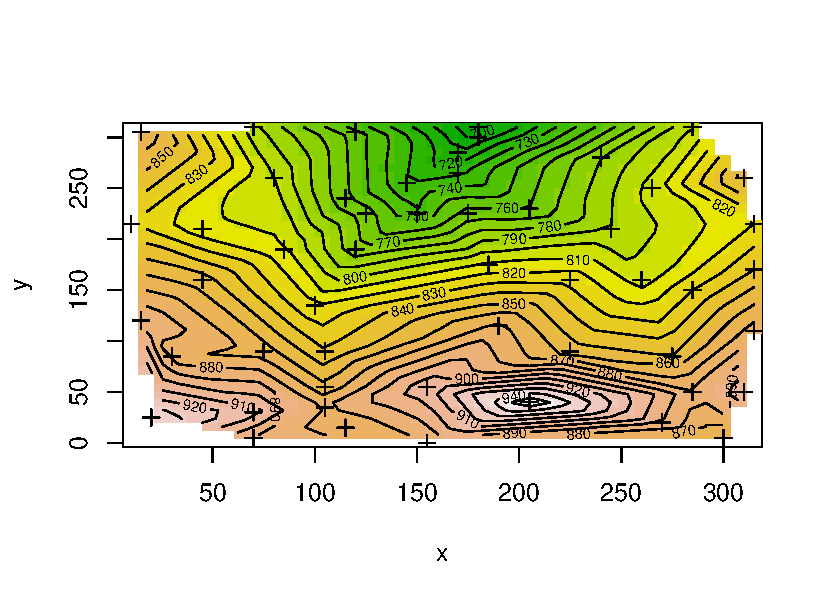
\includegraphics{figures/terrain2a.pdf}
    \caption{Contour plot with a heat-map of the interpolated observed data in $\mathcal{D}$}
    \label{fig:terrain2a}
\end{figure}


%%%%%%%%%%%%%%%%%%%%%%%%%%%%%%%%%%%%%%%%%%%%%%%%%%%%%%%%%%%%%%%%%%%%%%
\paragraph{b)}
Consider the continuous spatial variables $\{r(\vect{x}); \vect{x} \in \mathcal{D} \subset \mathbb{R}^2\}$ s.t.
\begin{equation}
\begin{array}{rcl}
     E[r(\vect{x})] & = & \vect{g}(\vect{x})^T\vect{\beta}_r \\
     \Var\{r(\vect{x})\} & = & \sigma_r^2 \\
     \Corr\{r(\vect{x}),r(\vect{x}^{'})\} & = & \rho_r(\vect{\tau}/\xi)
\end{array}
\end{equation}
with $\vect{g}(\vect{x}) = (g_1(\vect{x}), ... g_{n_g}(\vect{x}))$ a vector of known spatial variables and $\beta_r = (\beta_1, ..., \beta_{n_g})$ an unknown parameter. $\sigma_r^2 = 2500$ and the spatial correlation function have $\xi = 100$ with $\tau = |\vect{x} - \vect{x^{'}}|$. The prediction is 
\begin{equation}
    \hat{r}_0 = \vect{\alpha}^T\vect{r}_{n_g},
\end{equation}
with $\vect{\alpha} = (\alpha_1, ..., \alpha_{n_g})$ being the weights. 
The predictor error needs to be unbiased, which mean that the expected value of the error must be zero, giving
\begin{equation*}
\begin{array}{rcl}
    \E[\hat{r}_0 - r_0] & = & \vect{\alpha}^T \E[r^g]\\
      & \Downarrow & \\
      \vect{\alpha}^T \matr{G}_g \beta_r^+ & = & \vect{g}(\vect{x}_0) \\
      & \Downarrow & \\
      \matr{G}_g^T \vect{\alpha} & = & \vect{g}(\vect{x}_0)
\end{array}
\end{equation*}
with the ($n_g \times n_g$)-matrix $\matr{G}_g = (\vect{g}(\vect{x}_1,...,\vect{g}(\vect{x}_{n_g})^T$.
The optimization problem comes from minimizing the prediction error variance. It is derived from
\begin{equation*}
    \begin{array}{rcl}
        \vect{\hat{\alpha}} & = & \arg\min\limits_\alpha \Var\{\hat{r}_0 - r_0\} \\
         & = & \arg\min\limits_\alpha\{\sigma_r^2 - 2\vect{\alpha}^T\sigma_r^2\vect{\rho}_0 + \vect{\alpha}^T\sigma_r^2\matr{\Sigma}_g^\rho \vect{\alpha}\} \\
          & \textrm{constrained by} & \matr{G}_g^T \vect{\alpha} = \vect{g}(\vect{x}_0)
    \end{array}
\end{equation*}
The analytical solution using optimization with Lagrange multipliers is
\begin{equation*}
    \vect{\hat{\alpha}} = [\matr{\Sigma}_g^\rho]^{-1}\left[\vect{\rho}_0 - \matr{G}_g^T [\matr{G}_g[\matr{\Sigma}_g^\rho]^{-1}\matr{G}_g^T]^{-1}[\matr{G}_g[\matr{\Sigma}_g^\rho]^{-1}\vect{\rho}_0 - \vect{g}(\vect{x}_0)]\right],
\end{equation*}
which yields the universal kriging predictor and the associated prediction variance at an arbitrary location $\vect{x}_0 \in \mathcal{D}$.
\begin{equation}
    \begin{array}{rcl}
         \hat{r}_0 & = & \vect{\hat{\alpha}}^T \vect{r}_{n_g}  \\
         \sigma_{\hat{r}}^2 & = & \sigma_r^2\left[1-2\vect{\hat{\alpha}}^T \vect{\rho}_0 + \vect{\hat{\alpha}}^T\matr{\Sigma}_g^\rho \vect{\hat{\alpha}}\right] 
    \end{array}
\end{equation}
%%%%%%%%%%%%%%%%%%%%%%%%%%%%%%%%%%%%%%%%%%%%%%%%%%%%%%%%%%%%%%%%%%%%%%
\paragraph{c)}
Let the reference variable $\vect{x} \in \mathcal{D} \subset \mathbb{R}^2$ be $\vect{x} = (x_v, x_h)$ with $n_g = 6$, and the expectation function $\vect{g}(\vect{x}) = x_v^kx_h^l$ for $(k,l) \in \{(0,0),(1,0),(0,1),(1,1),(2,0),(0,2)\}$. Which means that the $n_g$-vector $\vect{g}(\vect{x}) = (1,x_v,x_h,x_vx_h,x_v^2,x_h^2)^T$. Looking at the expected value for $r(\vect{x})$ we get
\begin{equation*}
    \E[r(\vect{x})] = \vect{g}(\vect{x})^T \vect{\beta}_r = \beta_r^1 + x_v \beta_r^2 + x_h \beta_r^3 + x_v x_h \beta_r^4 + x_v^2 \beta_r^5 + x_h^2 \beta_r^6.
\end{equation*}
The values of $\vect{\beta}_r$ is unknown, but we don't need them to find the prediction. This is because of the unbiasedness of the expectation of the error in the prediction. 
The predicted value does not include the variance, and the variance does not include the actually values of the observations. 
In Figure \ref{fig:uk2} we see a heat map with contours of the predicted values $\hat{r}_{\vect{x}_0}$ and it resembles what we got in the interpolation made in Figure \ref{fig:terrain2a}. We also see the variance of the prediction, where the values are low close to the observed data points and higher far away from them. This is what we should expect from the formula of predicted variance.
\begin{figure}
\centering
    \begin{subfigure}[H]{0.99\textwidth}
        \centering
        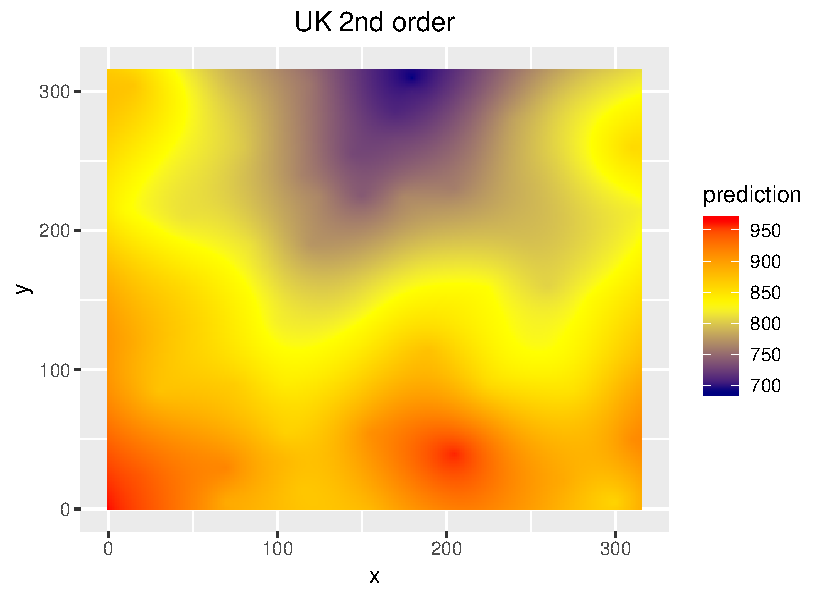
\includegraphics[scale=0.8,trim=0cm 0cm 0cm 0cm]{figures/uk2.pdf}
    \end{subfigure}
    \vskip\baselineskip
    \begin{subfigure}[H]{0.99\textwidth}  
        \centering 
        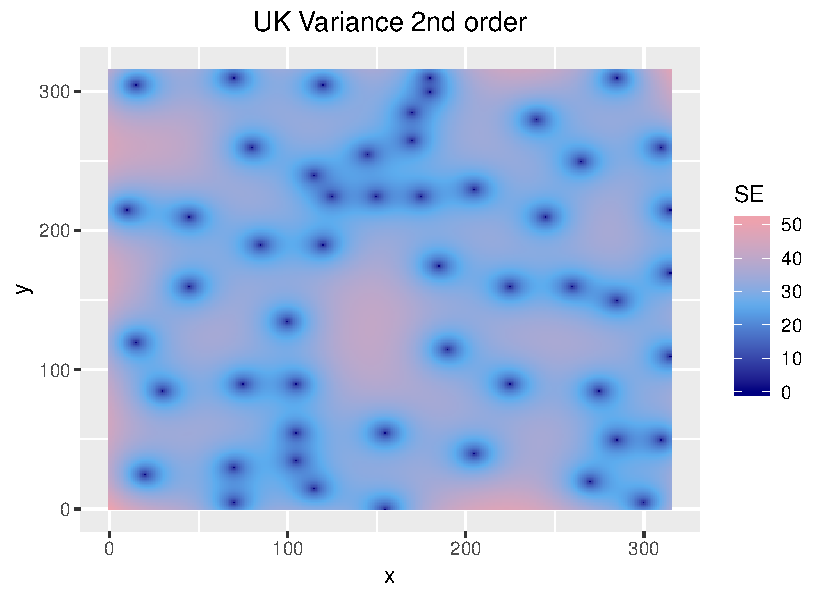
\includegraphics[scale=0.8,trim=0cm 0cm 0cm 0cm]{figures/uk2se.pdf}
    \end{subfigure}
    \caption{Top: Heat-map with contours of the predicted value $\hat{r}_{\vect{x}_0}$ on the grid $(0,315)\times(0,315)$ with second order expectation function. Bottom: Heat-map of the predicted variance $\sigma_{\hat{r}_{\vect{x}_0}}$ on a grid $(0,315)\times(0,315)$ with second order expectation function.}
    \label{fig:uk2}
\end{figure}
Now we consider the model with a 1st degree expectation function. Which means we remove the 2nd order terms from $\vect{g}(\vect{x})$. The comparison of the result is shown in Figure \ref{fig:uk1n2}. Here one can see a clear difference in predicted height between the models with 1st and 2nd degree expectation function. In the predicted variance you can't see much difference close to the data point, the further away the reference $\vect{x}_0$, the more difference one can observe. This also correlates with the deviations seen in the predicted value. The reason for this is that the 2nd degree terms of $\vect{\beta}_r$ is small and the difference in the variance of the 1st and 2nd degree model, is only visual when the variances gets large. Changing the variance $\sigma_r^2$ will off course change the variance in the model, but it doesn't change the predicted value.
\begin{figure}
\centering
    \begin{subfigure}[H]{0.99\textwidth}
        \centering
        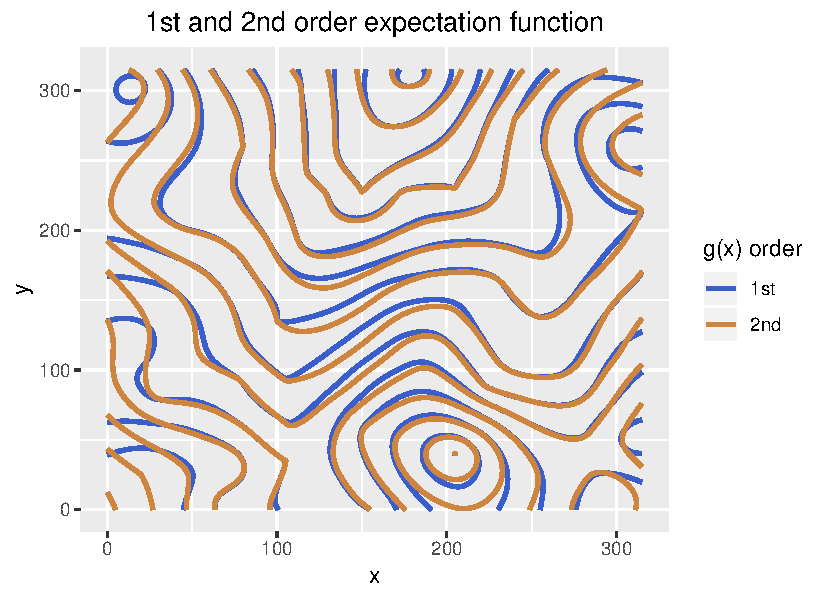
\includegraphics[scale=0.8,trim=0cm 0cm 0cm 0cm]{figures/uk1n2.pdf}
    \end{subfigure}
    \vskip\baselineskip
    \begin{subfigure}[H]{0.99\textwidth}  
        \centering 
        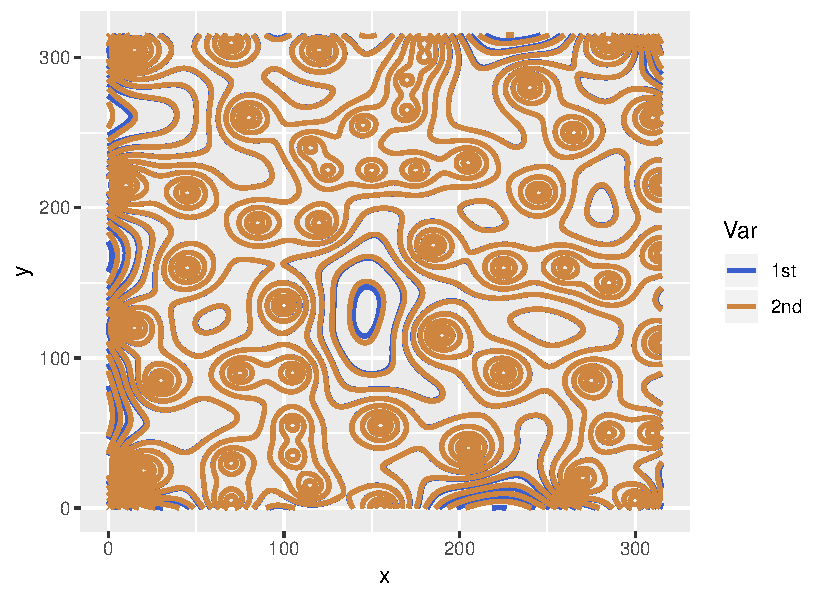
\includegraphics[scale=0.8,trim=0cm 0cm 0cm 0cm]{figures/uk1n2var.pdf}
    \end{subfigure}
    \caption{Top: A contour comparison of the predicted value with 1st and 2nd order expectation function $\vect{g}(\vect{x})$. Bottom: A contour comparison of the variance of the predicted variance with 1st and 2nd order expectation function.}
    \label{fig:uk1n2}
\end{figure}

%%%%%%%%%%%%%%%%%%%%%%%%%%%%%%%%%%%%%%%%%%%%%%%%%%%%%%%%%%%%%%%%%%%%%%
\paragraph{d)}
The probability for the height to be higher than 700 at the point $\vect{x}_0 = (100,100)$ is a normal distribution. The calculation yields 
\begin{equation*}
\begin{array}{cc}
     &  \\
     & 
\end{array}
    P\left(Z>\frac{700 - \hat{r}_{\vect{x}_0}}{\sigma_{\hat{r}_{\vect{x}_0}}}\right) = 1-P\left(Z\leq\frac{700 - \hat{r}_0}{\sigma_{\hat{r}_{\vect{x}_0}}}\right) = 1 - P\left(Z \leq \frac{700-838.2}{\sqrt{595.5}}\right)=1
\end{equation*}
So the probability for the height to be higher than 700 in $\vect{x}_0$ is 100\%.
The height at which the probability is 0.90 of the true height being lower than the predicted height at $\vect{x}_0$ is
\begin{equation*}
    Z|_{P = 0.9} = \frac{alt - \hat{r}_{\vect{x}_0}}{\sigma_{\hat{r}_{\vect{x}_0}}} = 1.28 \Rightarrow alt = 1.28\cdot \sqrt{595.5} + 838.2 =  869.4 .
\end{equation*}


%%%%%%%%%%%%%%%%%%%%%%%%%%%%%%%%%%%%%%%%%%%%%%%%%%%%%%%%%%%%%%%%%%%%%%
\paragraph{e)}
We want to look at the predicted value and variance when we add a observation error to the observation. The result from this is displayed in Figure \ref{fig:nugget}. Where you can see that this error doesn't change the predicted value, but in the variance you can see a clear difference. The predicted variance gets larger as the observation error gets larger, which is a natural response.
\begin{figure}
\centering
    \begin{subfigure}[H]{0.99\textwidth}
        \centering
        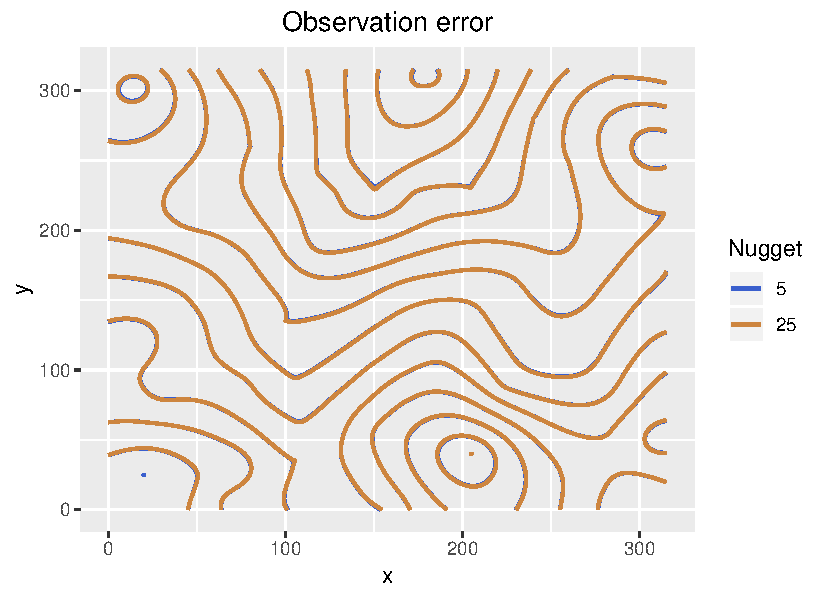
\includegraphics[scale=0.8,trim=0cm 0cm 0cm 0cm]{figures/nugget_pred.pdf}
    \end{subfigure}
    \vskip\baselineskip
    \begin{subfigure}[H]{0.99\textwidth}  
        \centering 
        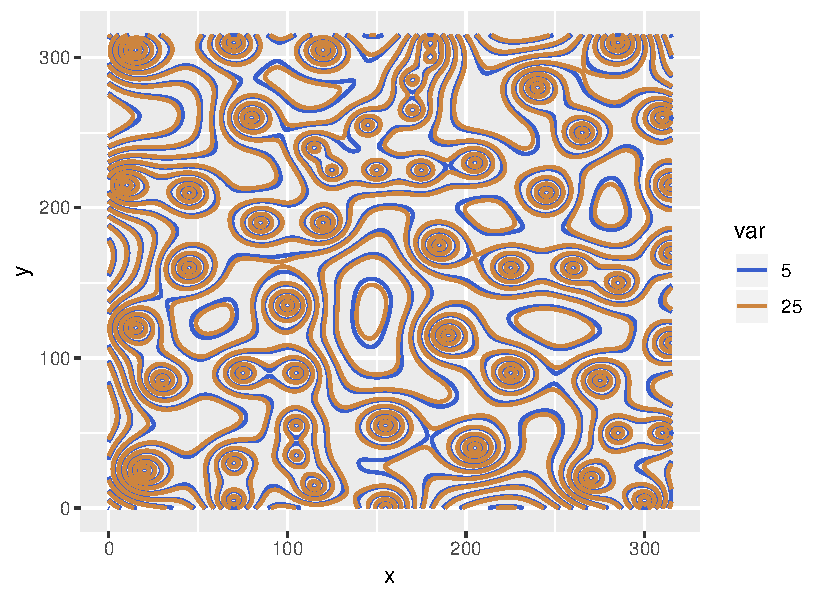
\includegraphics[scale=0.8,trim=0cm 0cm 0cm 0cm]{figures/nugget_var.pdf}
    \end{subfigure}
    \caption{Top: The predicted value of the observation with observation error. Bottom: predicted variance of the observation with observation error. The blue contours is $\sigma_\epsilon^2 = 5$ and the brown contours is $\sigma_\epsilon^2 = 25$ }
    \label{fig:nugget}
\end{figure}
%%%%%%%%%%%%%%%%%%%%%%%%%%%%%%%%%%%%%%%%%%%%%%%%%%%%%%%%%%%%%%%%%%%%%%
\paragraph{f)}
Using the kriging predictor formulated above, we achieved close to the same field of predicted values as with the interpolation. The $\beta$-values corresponding to the 2nd degree values of the expectation function was really small, so this resulted in a small difference in the prediction using a first degree expectation function. In the latter part of this exercise we introduced a observation error. This didn't affect the predicted value at all, but it resulted in a bigger predicted variance. 